\documentclass[11pt,onecolumn]{article}
\usepackage{amssymb, amsmath, amsthm,graphicx, subcaption, paralist,algpseudocode,algorithm,cancel,url,color}
\usepackage{sectsty}
\usepackage{fancyvrb}
\usepackage{mathrsfs}
\usepackage{multirow}
\usepackage{hhline}
\usepackage{booktabs}
\usepackage[table]{xcolor}
\usepackage{tikz}
% \usepackage[framed,numbered,autolinebreaks,useliterate]{mcode}
\usepackage{listings}
\usepackage{enumitem}
\usepackage{mathtools}

\newcommand{\bvec}[1]{\mathbf{#1}}
\newcommand{\R}{\mathbb{R}}
\newcommand{\C}{\mathbb{C}}
\newcommand{\Rn}{\R^{n\times n}}
\newcommand{\Rmn}{\R^{m\times n}}
\newcommand{\Cn}{\C^{n\times n}}
\newcommand{\Cmn}{\C^{m\times n}}
\newcommand{\cO}{\mathcal{O}}
\DeclareMathOperator{\Tr}{Tr}
\DeclareMathOperator{\trace}{trace}
\DeclareMathOperator{\diag}{diag}
\DeclareMathOperator{\vspan}{span}
\DeclarePairedDelimiter{\norm}{\|}{\|}
\DeclarePairedDelimiter{\abs}{|}{|}
\DeclarePairedDelimiter{\PAREN}{(}{)}
\sectionfont{\Large\sc}
\subsectionfont{\sc}
\usepackage[margin=1 in]{geometry}
\begin{document}
\noindent
\textsc{\Large Numerical analysis: P2}\\
Students: Bodong Liu (bl576), Ryan Wu (123123)\\
Date: May 3, 2025
\begin{center}\rule{1\linewidth}{0.5pt}\end{center}
\section*{Outline}
\begin{enumerate}
  \item \textbf{Introduction}

  \item \textbf{Optimization Methods}
    \begin{enumerate}
      \item Gradient Descent
      \item Quasi‑Newton (BFGS)
    \end{enumerate}

  \item \textbf{Small System Results}
    \begin{enumerate}
      \item $N=2$
      \item $N=3$
    \end{enumerate}
  
  \item \textbf{Convergence Analysis}

  \item \textbf{Discussion}

  \item \textbf{References}
\end{enumerate}

\newpage

\section{Introduction}
In this project, we are trying to solve the problem of finding lowest‐energy configurations of $N$ particles interacting according to a simplified version of Lennard–Jones potential in 3D space. We fix one particle to be translational invariant, optimizing the remaining $3(N-1)$ coordinates:
\[
  \min_{x_2,\ldots,x_N} \sum_{i=1}^{N-1}\sum_{j=i+1}^{N} V_{ij},
\]
where $r_{ij}=\|x_i - x_j\|$ and
\[
  V_{ij}(r) = r^{-12} - 2\,r^{-6}.
\]
Our goals are:
\begin{itemize}
  \item Implement two solver methods—Gradient Descent and a Quasi‑Newton BFGS—each with a backtracking line search and sensible stopping criteria.
  \item Validate these solvers by locating global minima for small systems ($N=2,3$) and argue uniqueness of the solutions.
  \item Analyze convergence behavior.
  \item Explore further how the solvers behave with greater $N$.
\end{itemize}

\section{Optimization Methods}

\subsection{Gradient Descent}
We implement the basic gradient descent method to minimize the Total Lennard–Jones Energy:
\[
  E(X) = \sum_{1\le i<j\le N} \Bigl(\|x_i - x_j\|^{-12} - 2\,\|x_i - x_j\|^{-6}\Bigr),
\]
working in the reduced \(3(N-1)\)-dimensional subspace by fixing \(x_1=(0,0,0)\). Below is a walkthrough of the core algorithm. Refer to Algorithm 1 in the "Algorithm" section for a more detailed pseudo-code.\\\\
\textbf {At each iteration \(k\):}

\begin{enumerate}
  \item \textbf{Compute gradient.}  
    \[
      g^{(k)} = \nabla E\bigl(X^{(k)}\bigr).
    \]
  \item \textbf{Line search (Armijo backtracking).}  Starting from \(\alpha = \alpha_0\), repeatedly shrink
    \(\alpha \leftarrow \beta\,\alpha\) until
    \[
      E\bigl(X^{(k)} - \alpha\,g^{(k)}\bigr)
      \;\le\;
      E\bigl(X^{(k)}\bigr)
      \;-\;
      c\,\alpha\,\|g^{(k)}\|^2,
    \]
    with default parameters \(\alpha_0=1.0\), \(\beta=0.5\), and \(c=10^{-4}\).
  \item \textbf{Update.}  
    \[
      X^{(k+1)} = X^{(k)} - \alpha\,g^{(k)}.
    \]
  \item \textbf{Stopping criteria.}
    \begin{itemize}
      \item {Gradient‐norm test:} \(\|g^{(k)}\|\le \epsilon_g\) (e.g.\ \(\epsilon_g=10^{-8}\)).
      \item {Maximum iterations:} \(k\ge K_{\max}\) (e.g.\ \(K_{\max}=2000\)).
      \item {Energy‐change test:} 
        \(\bigl|E(X^{(k+1)}) - E(X^{(k)})\bigr|\le\epsilon_E\).
    \end{itemize}
\end{enumerate}


\subsection{Quasi‑Newton (BFGS)}
We implement the BFGS method in the reduced subspace of dimension $3(N-1)$ by pinning one atom. Let $x^{(k)}$ and $g^{(k)}$ denote the free coordinates and gradient, and $H_k^{-1}$ the inverse‑Hessian approximation. Below is a general walkthrough for each iteration. Refer to Algorithm 2 in the "Algorithm" section for a more detailed pseudo-code.\\
\\
\noindent
\textbf {At each iteration \(k\):}
\begin{enumerate}
  \item \textbf{Compute full gradient.}  
    \[
      G^{(k)} = \nabla E\bigl(X^{(k)}\bigr),
      \quad
      g^{(k)} = \text{vec}\bigl(G^{(k)}\bigr)_{\rm free}.
    \]
  \item \textbf{Form search direction.}  
    \[
      s^{(k)} = -\,H_k^{-1}\,g^{(k)},
    \]
    where \(H_k^{-1}\in\mathbb R^{3(N-1)\times3(N-1)}\) is our current inverse‑Hessian approximation.
  \item \textbf{Line search (Armijo backtracking).}  
    Choose \(\alpha=\alpha_0\) and shrink \(\alpha\leftarrow\beta\,\alpha\) until
    \[
      E\bigl(X^{(k)} + \alpha\,S^{(k)}\bigr)
      \;\le\;
      E\bigl(X^{(k)}\bigr)
      -c\,\alpha\,\bigl(g^{(k)}\bigr)^\top s^{(k)},
    \]
    where \(S^{(k)}\) is \(s^{(k)}\) re‑inserted into the full coordinate vector.  Default parameters: \(\alpha_0=1\), \(\beta=0.5\), \(c=10^{-4}\).
  \item \textbf{Update iterate.}
    \[
      x^{(k+1)} = x^{(k)} + \alpha\,s^{(k)},
      \quad
      X^{(k+1)} = \text{assemble}(x^{(k+1)}),
      \quad
      X^{(k+1)}.\mathrm{requires\_grad\_()} = \texttt{True}.
    \]
  \item \textbf{Compute new gradient.}  
    \[
      G^{(k+1)} = \nabla E\bigl(X^{(k+1)}\bigr),
      \quad
      g^{(k+1)} = \text{vec}\bigl(G^{(k+1)}\bigr)_{\rm free}.
    \]
  \item \textbf{BFGS update.}  
    Form
    \[
      y^{(k)} = g^{(k+1)} - g^{(k)},\quad
      \rho^{(k)} = \frac{1}{(y^{(k)})^\top s^{(k)}}.
    \]
    \begin{itemize}
      \item If \((y^{(k)})^\top s^{(k)} < 10^{-8}\), skip update (to avoid a non‑positive or numerically unstable \(\rho\)).
      \item Otherwise,
        \[
          V = I - \rho^{(k)}\,s^{(k)} (y^{(k)})^\top,\quad
          H_{k+1}^{-1}
          = V\,H_k^{-1}\,V^\top
            + \rho^{(k)}\,s^{(k)} (s^{(k)})^\top.
        \]
    \end{itemize}
  \item \textbf{Stopping criteria.}
    \begin{itemize}
      \item {Energy‐change test:} 
        \(\bigl|E(X^{(k+1)}) - E(X^{(k)})\bigr|\le\epsilon_E\).
      \item {Gradient‐norm test:} 
        \(\|g^{(k+1)}\|\le\epsilon_g\).
      \item {Maximum iterations:} \(k\ge K_{\max}\).
    \end{itemize}
\end{enumerate}

% Result
\section{Small Systems Results}

In this section we apply our Gradient Descent and BFGS implementations to the cases \(N=2\) and \(N=3\).  We report the found configurations, energies, and argue for global optimality and uniqueness.

\subsection{\(N=2\)}

\paragraph{Expected solution:}  
With only two atoms and the simplified L-J potential
\[
  V(r) = r^{-12} - 2\,r^{-6},
\]
we can hand-calculate and obtain the unique minimizer:
\[
  r^* = 1,\qquad V(r^*) = -1.
\]

\paragraph{Computed result:}
Our GD solver converges to
\[
  X =
  \begin{bmatrix}
    (0,0,0) \\[3pt]
    (0.7923309,\,-0.3080589,\,0.5266037)
  \end{bmatrix}, \quad
  r_{12} \approx 1,
  \quad
  E(X) \approx -1.0000.
\]


Our BFGS solver converges to
\[
  X =
  \begin{bmatrix}
    (0,0,0) \\[3pt]
    (-0.7923317,\,0.3080592,\,-0.5266043)
  \end{bmatrix}, \quad
  r_{12} \approx 1,
  \quad
  E(X) \approx -1.0000.
\]

% N22222
Two solvers produce identical geometry as below.
\begin{figure}[h]
  \centering
  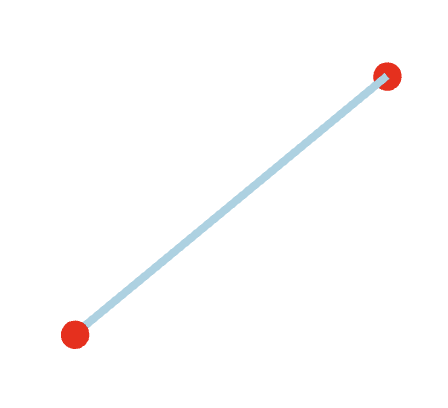
\includegraphics[width=0.4\textwidth]{N2.png}
  \caption{Configuration for \(N=2\).}
\end{figure}

\paragraph{Global optimality and uniqueness:}  
Since there is only one pair interaction, the derivative of potential energy has a single critical point at \(r=1\), which is a global minimum.  Hence, this minimization is unique (not counting rotation or translation).

\subsection{\(N=3\)}

\paragraph{Expected solution:}  
For three atoms, symmetry suggests an equilateral triangle of side length \(r^*=1\).  The total energy is
\[
  E_3 = 3\,V(1) = -3.
\]

\paragraph{Computed result:}  
Our GD solver converges to:,
\[
  X \approx
  \begin{bmatrix}
    (0,0,0) \\[3pt]
    (-0.8421267,\,0.3627993,\,-0.3989978) \\[3pt]
    (-0.4070932,\,-0.444385,\,-0.7979956)
  \end{bmatrix}, \quad
  r_{ij} \approx 1 \quad \forall 1\leq i<j \leq3,
  \quad
  E(X) \approx -3.0000.
\]

Our BFGS solver converges to:,
\[
  X \approx
  \begin{bmatrix}
    (0,0,0) \\[3pt]
    (-0.8421709,\,0.3649025,\,-0.3969839) \\[3pt]
    (-0.4092407,\,-0.4424151,\,-0.7979930)
  \end{bmatrix}, \quad
  r_{ij} \approx 1 \quad \forall 1\leq i<j \leq3,
  \quad
  E(X) \approx -3.0000.
\]

% N33333
Two solvers produce identical geometry. As we can see from below that the configuration is a equilateral triangle which matches the theoretical solution.
\begin{figure}[h]
  \centering
  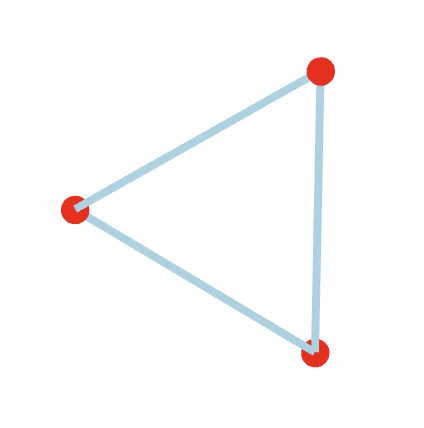
\includegraphics[width=0.5\textwidth]{N3.png}
  \caption{Configuration for $N=3$}
\end{figure}

\paragraph{Global optimality and uniqueness.}  
By symmetry and convexity of the sum of identical pairwise interactions, the equilateral triangle is the configuration that minimizes \(\sum_{i<j}V(\|x_i-x_j\|)\).  There are no other forms of triangles achieving \(E=-3\).  Hence, this minimization is unique (not counting rotation or translation).

\newpage
% Cnonvegence
\section{Convergence Analysis}
\subsection{Gradient Descent}

In a three atom configuration, we found that globally optimal configurations for N=3 for the gradient descent implementation using line search converges roughly linearly, and in a low numnber of steps. The follows shows the estimated convergence order, where $error_{n}$ is the absolute difference of energy between the $n-1$ and $n$ iterations. 

\begin{figure}[h]
  \centering
  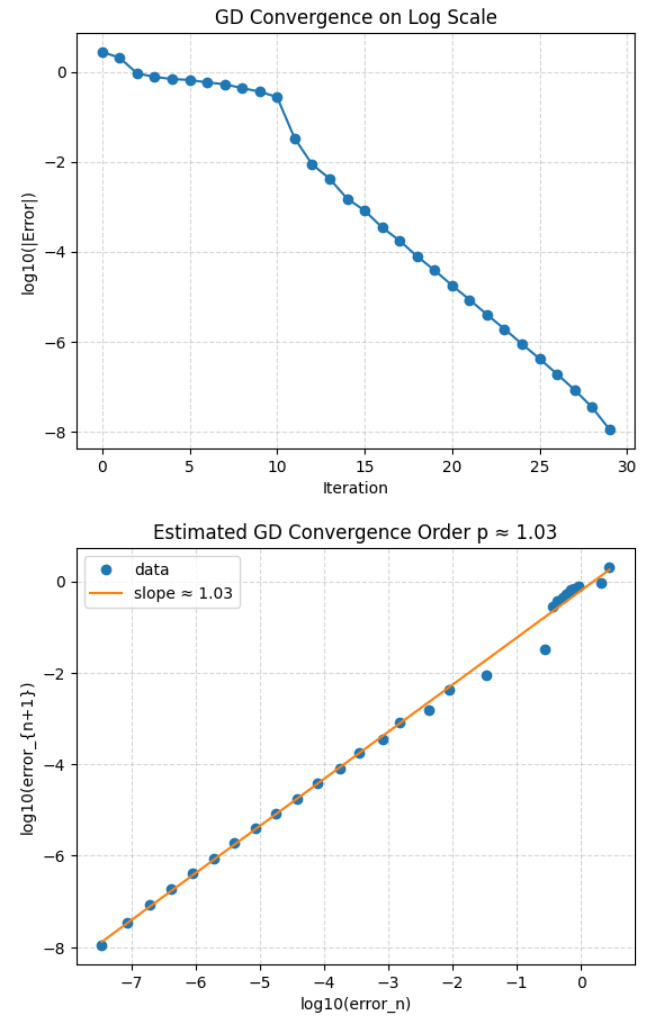
\includegraphics[width=0.5\textwidth]{./GD_conv_uniform.png}
  \caption{Convergence for Gradient Descent, N=3}
\end{figure}


\noindent
These fall in line with our expectations for the performance of Gradient Descent, where it typically has a linear convergence rate (our experimental convergence rate is $\rho=1.03$).

\subsection{BFGS}

The theoretical order of convergence of BFGS is Q-superlinear, where it should converge faster than linear in specific conditions. However, the conditions for this case are rather strong: the Hessian must be positive definite in the neighborhood of the minimzer, the line serach much satisfy the strong Wolfe conditions, and the problem is non-degenerate. 

% Discussion
\section{Discussion}
We ran both solvers for greater values of $N$ up to $N=10$ as reported in Table 1. We also included the simulation results from The Cambridge Cluster Database in the last column to have a better look at how good our solvers are. The Cambridge Cluster Database uses a 'basin-hopping' algorithm for $N<110$, which are unbiased global optimization methods (The Cambridge Cluster Database). We can see that our solvers are generally doing great. The biggest discrepancy occurs at $N=10$ with an error of $5.8\%$.

% Table
\begin{table}[h]
\centering
\begin{tabular}{|c|c|c|c|}
\hline
\(N\) & \(E(\mathrm{GD})\) & \(E(\mathrm{BFGS})\) & \(E(\mathrm{Cambridge)}\) \\ \hline
4  & -6.000000  & -6.000000  & -6.000000  \\ \hline
5  & -9.103852  & -9.103852  & -9.103852 \\ \hline
6  & -12.712062 & -12.302927 & -12.712062 \\ \hline
7  & -16.505384 & -16.505384 & -16.505384 \\ \hline
8  & -19.765298 & -19.765297 & -19.821489\\ \hline
9  & -23.269812 & -23.269812 & -24.113360\\ \hline
10 & -26.771677 & -26.771677 & -28.422532\\ \hline
\end{tabular}
\caption{Results from Gradient Descent, BFGS, and The Cambridge Cluster Database}
\end{table}

\noindent In our initial version of BFGS algorithm, we observed the total energy and gradient norm become NaN after a few iterations.  It was because  
\[
  y^{(k)\top}s^{(k)} 
  = \bigl(g^{(k+1)}-g^{(k)}\bigr)^\top s^{(k)}
\]
could become extremely small or even slightly negative when the gradient does not change much plus the numerical noise and inexact line searches.  Since the BFGS update uses  
\(\rho = 1/(y^Ts)\), a tiny or non‑positive denominator sends \(\rho\) to huge or undefined values, which in turn causes the inverse Hessian to be not positive definiteness and leads to NaN steps.  To fix this, we insert the safeguard  
\[
  \text{if }y^{(k)\top}s^{(k)} \le 10^{-8}, \quad\text{skip the BFGS update.}
\]
This simple check prevents dividing by (near) zero, preserves positive‑definiteness of the Hessian estimate, and immediately stops the pathological growth in subsequent iterates—eliminating the NaNs and restoring reliable convergence.  


\((y^{(k)})^\top s^{(k)} < 10^{-8}\)

% Images of N>4
\begin{figure}[h]
  \centering
  \begin{subfigure}[b]{0.45\textwidth}
    \centering
    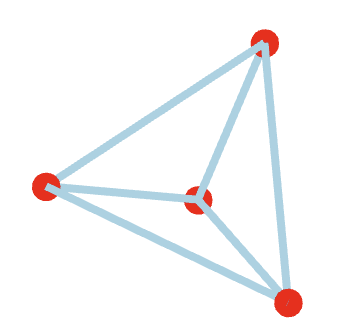
\includegraphics[width=0.45\textwidth]{N4.png}
    \caption{N=4}
    \label{fig:sub1}
  \end{subfigure}
  \hfill
  \begin{subfigure}[b]{0.45\textwidth}
    \centering
    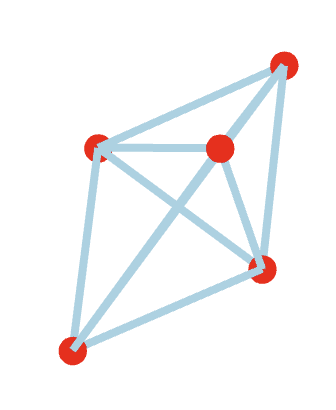
\includegraphics[width=0.45\textwidth]{N5.png}
    \caption{N=5}
    \label{fig:sub2}
  \end{subfigure}

  \vspace{1em}

  \begin{subfigure}[b]{0.45\textwidth}
    \centering
    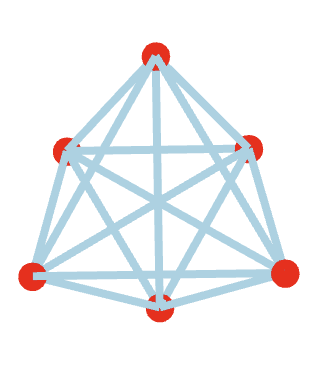
\includegraphics[width=0.45\textwidth]{N6_1.png}
    \caption{N=6 (GD)}
    \label{fig:sub3}
  \end{subfigure}
  \hfill
  \begin{subfigure}[b]{0.45\textwidth}
    \centering
    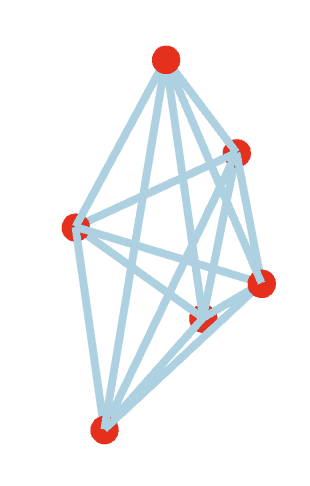
\includegraphics[width=0.45\textwidth]{N6_2.png}
    \caption{N=6 (BFGS)}
    \label{fig:sub4}
  \end{subfigure}

  \vspace{1em}

  \begin{subfigure}[b]{0.45\textwidth}
    \centering
    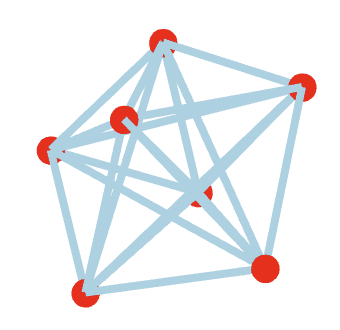
\includegraphics[width=0.45\textwidth]{N7.png}
    \caption{N=7}
    \label{fig:sub3}
  \end{subfigure}
  \hfill
  \begin{subfigure}[b]{0.45\textwidth}
    \centering
    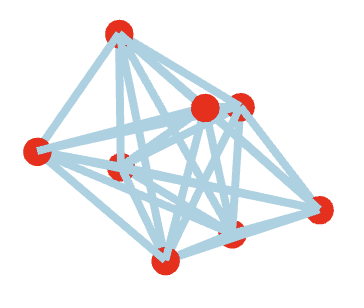
\includegraphics[width=0.45\textwidth]{N8.png}
    \caption{N=8}
    \label{fig:sub4}
  \end{subfigure}

  \vspace{1em}

  \begin{subfigure}[b]{0.45\textwidth}
    \centering
    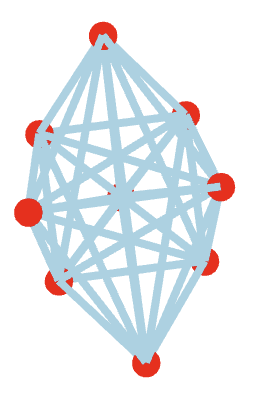
\includegraphics[width=0.45\textwidth]{N9.png}
    \caption{N=9}
    \label{fig:sub3}
  \end{subfigure}
  \hfill
  \begin{subfigure}[b]{0.45\textwidth}
    \centering
    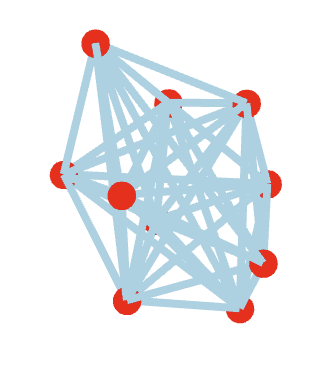
\includegraphics[width=0.45\textwidth]{N10.png}
    \caption{N=10}
    \label{fig:sub4}
  \end{subfigure}

  \caption{Geometries for $N=4,5,6,7,8,9,10$.}
  \label{fig:grid}
\end{figure}


% Algorithm
\newpage
\section{Algorithm Pseudo-code}
We referenced the textbook for help with generating the pseudo algorithm (Ascher et al., 2011).
\begin{algorithm}[H]
\caption{Gradient Descent}
\begin{algorithmic}[1]
\Require initial $X^{(0)}$, parameters $\alpha_0, \beta, c$, tolerances $\epsilon_g, \epsilon_E$, max iter $K$
\For{$k=0$ to $K-1$}
  \State compute $g^{(k)} = \nabla E(X^{(k)})$
  \State $\alpha \gets \alpha_0$
  \While{$E(X^{(k)} - \alpha\,g^{(k)}) > E(X^{(k)}) - c\,\alpha\,\|g^{(k)}\|^2$}
    \State $\alpha \gets \beta\,\alpha$
  \EndWhile
  \State $X^{(k+1)} \gets X^{(k)} - \alpha\,g^{(k)}$
  \If{$\Delta E\leq \epsilon_E$ or $\|g^{(k)}\| \le \epsilon_g$} 
    \State break \Comment{delta-energy, gradient-norm guard}
  \EndIf
\EndFor
\end{algorithmic}
\end{algorithm}
\begin{algorithm}[H]
\caption{BFGS}
\begin{algorithmic}[1]
\Require initial $X^{(0)}$, free vector $x^{(0)}$, $H_0^{-1}=I$, parameters $\alpha_0, \beta, c$, tolerances $\epsilon_g, \epsilon_E$, max iter $K$
\For{$k=0$ to $K-1$}
  \State compute full gradient $g^{(k)} = \nabla E(X^{(k)})$
  \State extract free gradient $g^{(k)}_{\rm free}$
  \If{$\|g^{(k)}_{\rm free}\| \le \epsilon_g$}
    \State break \Comment{gradient‑norm guard}
  \EndIf
  \State $s^{(k)} \gets -H_k^{-1}\,g^{(k)}_{\rm free}$
  \State Armijo line search to find $\alpha_k$
  \State $x^{(k+1)} \gets x^{(k)} + \alpha_k\,s^{(k)}$
  \State assemble $X^{(k+1)}$ from free $x^{(k+1)}$, reenable gradient tracking
  \State compute $g^{(k+1)}_{\rm free}$
  \State $y^{(k)} \gets g^{(k+1)}_{\rm free} - g^{(k)}_{\rm free}$
  \If{$(y^{(k)})^T s^{(k)} < 10^{-8}$}
    \State skip BFGS update
  \Else
    \State $\rho = 1 / ((y^{(k)})^T s^{(k)})$
    \State $V = I - \rho\,s^{(k)}(y^{(k)})^T$
    \State $H_{k+1}^{-1} = V\,H_k^{-1}\,V^T + \rho\,s^{(k)}(s^{(k)})^T$
  \EndIf
  \State $\Delta E = |E(X^{(k+1)}) - E(X^{(k)})|$
  \If{$\Delta E \le \epsilon_E$}
    \State break \Comment{delta-energy guard}
  \EndIf
\EndFor
\end{algorithmic}
\end{algorithm}

\newpage
\section{References}
The Cambridge Cluster Database, D. J. Wales, J. P. K. Doye, A. Dullweber, M. P. Hodges, F. Y. Naumkin F. Calvo, J. Hernández-Rojas and T. F. Middleton, URL http://www-wales.ch.cam.ac.uk/CCD.html.\\

Ascher, U. M., \& Greif, C. (2011). A first course in numerical methods. SIAM, Society for Industrial and Applied Mathematics. 


\end{document}
